\section{Effektive Masse - Rückblick auf Mikro 1+2}
Die Beschreibung der Eigenleitung wird unter der Annahme getroffen, dass ein Elektron sich frei im Kristallgitter bewegen könne. Tatsächlich wirken aber innere Kräfte des Kristallgitters auf das Elektron. Diese Wirkung wird durch die Einführung einer effektiven Masse kompensiert.
	\begin{equation}
		m^* = \underbrace{\alpha}_{const.} \cdot \underbrace{m_0}_{Elektr. Masse} \qquad ,\; \alpha < 1,\; \text{materialabhängig}
	\end{equation}

\section{Halbleitertypen}
	\subsection{Halbleiter und Metalle}
	\begin{itemize}
		\item Metalle sind grundsätzlich Kaltleiter $\rightarrow$ $T=0K \; \Rightarrow \; \sigma_M \rightarrow \infty$
		\begin{itemize}
			\item T $\uparrow \Rightarrow \sigma_M \downarrow, \; \sigma_M >>0$
		\end{itemize}
		\item Halbleiter sind grundsätzlich Heissleiter
		\begin{itemize}
			\item $T\uparrow \Rightarrow \sigma_{HL} \uparrow, \text{ aber } \sigma_{HL} << \sigma_M$
		\end{itemize}
	\end{itemize}
	
	\subsection{Elementhalbleiter} \label{ss_hltyp_ehl}
	Elementhalbleiter sind Halbleiter die nur aus einem Element bestehen.
	\subsection{Verbindungshalbleiter} \label{ss_hltyp_vhl}
	Verbindungshalbleiter sind immer 50/50 aufgeteilt, d.h. am Beispiel eines GaN (Galliumnitrid) III-V Verbindungshalbleiter ist das Kristallgitter so aufgebaut dass au jedes Galliumatom ein Stickstoffatom und dann wieder ein Galliumatom folgt. 
	\subsection{Legierungshalbleiter} \label{ss_hltyp_lhl}
	Legierungshalbleiter sind im Gegensatz zu Verbindungshalbleiter beliebig mischbar. Grundsätzlich sind alle Verhältnisse denkbar die sich ineinander lösen lassen.So können auch Kristallgitter entstehen, in denen gleiche Atome direkt benachbart sind.
	
\section{Bindungsarten}
	\subsection{Elektronenpaarbindung}
	Die zentrale Bindung bei Halbleitern ist die kovalente Bindung (auch Elektronenpaarbindung genannt). Aus \ref{ss_hltyp_lhl} und \ref{ss_hltyp_ehl} erkennt man damit, dass bei Verbindungshalbleitern nur kovalente Bindungen zwischen unterschiedlichen Atomen vorkommen kann, also am Beispiel von vorher nur kovalente Bindungen zwischen Gallium udn Stickstoff. Bei Legierungshalbleitern können dagegen auch kovalente Bindungen zwischen selben Atomen vorkommen, zum Beispiel Si-Si (Silizium) oder Ca-Ca (Cadmium) kovalente Bindungen.
	Kovalente Bindungen basieren auf dem Spin der äusseren Elektronen. Da bei der kovalenten Bindung beide Elektronen von jeweils beiden Atomen als äussere Elektronen beansprucht werden müssen die Spins entgegengesetzt sein. Damit ist das magnetische Moment entgegengesetzt wodurch eine magnetische Bindung entsteht. Es lässt sich so auch das heissleitende Verhalten von Halbleitern begründen. Bei $T=0K$ herrscht absolut keine Bewegung im Kristall. Entsprechend trennen sich die kovalenten Bindungen ohne weitere Krafteinwirkung nicht auf und damit verhält sich das Material wie ein Isolator. Steigt die Temperatur an beginnen die Ionen und Elektronen sich zu bewegen. So kann es passieren dass sich einzelne kovalente Bindungen aufbrechen.
	\subsection{Metallische Bindung}
	Bei einem Metall gehört jedes Valenzelektron zu sehr vielen Atomen, somit verteilt sich die Bindung über das gesamte Volumen. Man kann sich ein Metall strukturell als Raumgitter aus vielen positiven Ionen vorstellen, zwischen denen sich ein frei bewegliches Elektronengas befindet. Diese freien Elektronen bilden somit eine negative Ladungswolke. Die Wechselwirkung aus der negativen Ladungswolke und den positiven Gitterionen sind Grundlage für die metallische Bindung. Typischerweise gibt jedes Atom ein bis zwei Atome in das Elektronengas, auch Fermi-Gas oder Fermi-See genannt, ab. Damit kann man direkt abschätzen, dass die Anzahl freier Elektronen zwar von Metall zu Metall variiert, aber in der Größenordnung immer ähnlich zur Anzahl der Atome sein muss.
	\subsection{Ionische Bindung}
	Grundsätzlich sind Atome bestrebt Edelgaskonfiguration anzunehmen, d.h. ihre äußerste Schale mit 8 Aussenelektronen zu besetzen. Eine ionische Bindung kommt dann besonders leicht zustande, wenn ein Atom zum Beispiel Natrium ein Aussenelektron in der äußersten Schale hat in räumliche Nähe zu einem weiteren Atom kommt dem gerade ein Aussenelektron zur Edelgaskonfiguration fehlt, z.B. Chlor. Gibt das Natrium sein Aussenelektron ab so ist die "neue" äußerste Schale gerade voll besetzt. Nimmt Chlor das abgegebene Elektron auf, so ist seine äußerste Schale auch gerade voll besetzt. Das Natriumatom wird damit zu einem positiv geladenen Natriumion, das Cloratom zu einem negativ geladenen Chloridion, die beide in Edelgaskonfiguration sind. Diese Verbindung heißt Natriumchlorid. Eine ionische Bindung kann aber auch in der Form vorliegen dass ein Atom mehrere Elektronen in der äußersten Schale hat. Aluminium hat zum Beispiel 3 Elektronen in der äußersten Schale, die es abgeben müsste um Edelgaskonfiguration zu erreichen. Es wäre dann ein 3-fach positiv geladenes Aluminiumion. Um diese Konfiguration zu erreichen muss es sich mit 3 Chloratomen verbinden, da jedes Chloratom bestrebt ist nur ein Elektron aufzunehmen. Die so entstandene Verbindung heißt Aluminiumchlorid.
	
	\section{Bandstruktur}
	Es existieren 2 Arten von Bandstruktur, zum einen die bekannte elektrische Bandstruktur, zum anderen die photonische Bandstruktur, über die z.B. ein Halbleiter unter Lichteinfluss beschrieben werden kann. Grundsätzlich muss aber beachtet werden, dass die Bandstruktur ein menschengemachtes Werkzeug ist um die Vorgänge im Material zu visualisieren und begreifen zu können. Folgend einige Graphiken unterschiedlicher Darstellungsmöglichkeiten der Vorgänge im Halbleiter:
\begin{figure}[H]
	\begin{minipage}{.5\linewidth}
		\centering
		\subfloat[]{\label{main:a}\includegraphics[scale=.2]{./img/bandstr_ul.png}}
	\end{minipage}%
	\begin{minipage}{.5\linewidth}
		\centering
		\subfloat[]{\label{main:c}\includegraphics[scale=.2]{./img/bandstr_or.png}}
	\end{minipage}\par\medskip
	\centering
	\subfloat[]{\label{main:b}\includegraphics[scale=.23]{./img/bandstr_ur.png}}
	\caption{Darstellungsformen \protect\cite{HL1}}
\label{fig:bandstr_darstell}
\end{figure}

(a) ist eine geschickte 2-dimensionale Darstellung von (c). Die in eckigen Klammern angegebenen Zahlenkombinationen nennt man Miller Indizies. (b) zeigt die Fermi-Fläche von Kupfer.\newline
Die Bandstruktur eines Materials ist ein Modell der erlaubten Impulse und der erlautebn Orte, sowie der jeweiligen Gesamtenergie. Damit ergeben  sich 7 Dimensionen die entsprechend nicht darstellbar sind. Man teilt die Struktur daher in zwei Räume ein. Den Ortsraum und den Impulsraum. In beiden Räumen stehen so 3 Dimensionen zur Verfügung. Die Gesamtenergie wird dann oft zusätzlich farblich dargestellt wie auch in \ref{fig:bandstr_darstell} (b) zu sehen ist. Dies gibt erste Indizien über den Zusammenhang zwischen Teilchen und Welle. Der Impuls ist klassisch gegeben mit
\begin{equation}
	\vec{p} = m\vec{v}
\end{equation}
und lässt sich als Betrag auch schreiben als
\begin{equation}
	|\vec{p}| = \frac{h}{\lambda}
\end{equation}
mit $h$ als Planksche Konstante und $\lambda$ als Wellenlänge. Vektoriell lässt sich der Zusammenhang mit dem Wellenvektor $\vec{K}$ wie folgt ausdrücken:
\begin{align}
	\vec{K} &= \vecT{K_x \\ K_y \\ K_z} \\
	\vec{p} &= \hbar \vec{k} \\
	 |\vec{K}| :&= \frac{2 \pi}{\lambda}
\end{align}
Bei der Behandlung von Wellen ist immer zu beachten, dass die entscheidenden Größen zur Beschreibung einer Welle die Frequenz $f$, die Wellenlänge $\lambda$ und die Intensität  $I$.

Zur Vereinfachung betrachtet man zunächst kubisch primitive Kristalle. Unter einer primitiven Elementarzelle versteht man eine Zelle, in der nur an den Ecken jeweils Atome sind. Dies ist zum Beispiel bei einem Metall durch die Metallionen gegeben.

\begin{figure}[H]
	\begin{minipage}{.5\linewidth}
		\centering
		\subfloat[]{\label{main:a}\includegraphics[scale=.2]{./img/bandstr_kubPrim_a.png}}
	\end{minipage}%
	\begin{minipage}{.5\linewidth}
		\centering
		\subfloat[]{\label{main:c}\includegraphics[scale=.2]{./img/bandstr_kubPrim_a.png}}
	\end{minipage}\par\medskip
	\caption{Bandstruktur Metall \protect\cite{HL1}}
\label{fig:bandstr_kubPrim_a}
\end{figure}

Als erster Ansatz kann man versuchen die Gesamtenergie im System klassisch zu berechnen:
\begin{align}
	E_{ges} &= E_{kin,ges} + E_{pot,ges} \nonumber \\
	&= \sum\limits_{i=1}^N \frac{1}{2}m|\overset{\cdot}{\vec{r_i}}|^2 + \sum\limits_{i=1}^N \frac{1}{2}m|\overset{\cdot}{\vec{R_i}}|^2 + \underset{i \neq j}{\sum\limits_{i,j=1}^N} \frac{1}{4 \pi \varepsilon_0 \varepsilon_r} \cdot \frac{(-q)^2}{|\vec{r_i} - \vec{r_j}|}+ \underset{i \neq j}{\sum\limits_{i,j=1}^N} \frac{1}{4 \pi \varepsilon_0 \varepsilon_r} \cdot \frac{(-q)^2}{|\vec{R_i} - \vec{R_j}|} \nonumber\\ &\qquad \qquad \qquad \qquad \qquad \qquad + \sum\limits_{i,j=1}^N \frac{1}{4 \pi \varepsilon_0 \varepsilon_r} \cdot \frac{(-q)^2}{|\vec{r_i} - \vec{R_j}|}
\end{align}
Dieser Ansatz führt aber zwangsläufig zu Fehler da hiernach sämtliche Bahnradien zulässig wären was jedoch dem dritten Bohrschen Postulat widerspricht.
Wie lässt sich dennoch eine Beschreibung mit Hilfe der Bohrschen Postulate und bekanntem Wissen für das Verhalten im Metallgitter? Zur Vereinfachung nimmt man einen Schnitt aus einem kubischen Kristall, hier wieder das Beispiel metallischer Bindung und strippt das Gitter sodass nur noch die Metallionen übrig bleiben (siehe \ref{fig:bandstr_metallg_a}). Mann kann sich nun phänomenologisch überlegen, welche Orte für die Elektronen zulässig wären. Je näher der Bahnradius am Mutterkern liegt, desto stärker wirkt die Anziehung des Kerns aufs Elektron. Das heißt in unmittelbarer Nachbarschaft zum Kerns ist die dominante Kraft die Anziehung zum Mutterkern, die Kräfte der anderen benachbarten Kerne werden zwar auch vom Elektron gespürt, sind aber nicht stark genug um es aus dem bohrschen Radius zu reissen. Im Beispiel \ref{fig:bandstr_metallg_b} sind die ersten zwei bohrschen Radien entsprechende Radien die ausreichend fest gebunden sind. Dazwischen ergeben sich die klassischen nichtbesetzbaren Radien (in \ref{fig:bandstr_metallg_b} weiß dargestellt). Je weiter sich nun der Radius vom Kern entfernt, desto verhältnismäßig stärker wirken die Kräfte der Nachbaratome auf das Elektron. Ab einem gewissen Punkt ist das Elektron so weit vom Mutterkern entfernt, dass die Kraftunterschiede so gering sind, dass es sehr leicht von der Anziehung vom Mutterkern entfernt werden kann. So ergibt sich ein großer, verbundener Bereich besetzbarer Gebiete, der Fermi-See (in \ref{fig:bandstr_metallg_b} blau dargestellt).

\begin{figure}[H]
	\begin{minipage}{.5\linewidth}
		\centering
		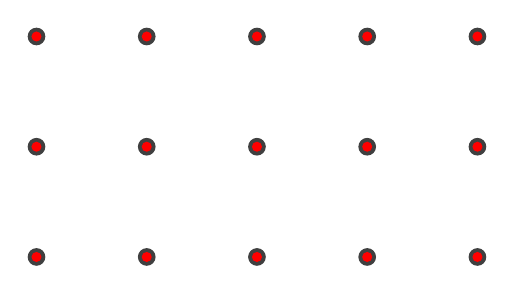
\begin{tikzpicture}[scale=0.7]
		\draw[fill, darkgray] (2,6) circle [radius=0.15];
		\draw[fill, red] (2,6) circle [radius=0.08];
		\draw[fill, darkgray] (2,4) circle [radius=0.15];
		\draw[fill, red] (2,4) circle [radius=0.08];
		\draw[fill, darkgray] (2,2) circle [radius=0.15];
		\draw[fill, red] (2,2) circle [radius=0.08];
		
		\draw[fill, darkgray] (4,6) circle [radius=0.15];
		\draw[fill, red] (4,6) circle [radius=0.08];
		\draw[fill, darkgray] (4,4) circle [radius=0.15];
		\draw[fill, red] (4,4) circle [radius=0.08];
		\draw[fill, darkgray] (4,2) circle [radius=0.15];
		\draw[fill, red] (4,2) circle [radius=0.08];
		
		\draw[fill, darkgray] (6,6) circle [radius=0.15];
		\draw[fill, red] (6,6) circle [radius=0.08];
		\draw[fill, darkgray] (6,4) circle [radius=0.15];
		\draw[fill, red] (6,4) circle [radius=0.08];
		\draw[fill, darkgray] (6,2) circle [radius=0.15];
		\draw[fill, red] (6,2) circle [radius=0.08];
		
		\draw[fill, darkgray] (8,6) circle [radius=0.15];
		\draw[fill, red] (8,6) circle [radius=0.08];
		\draw[fill, darkgray] (8,4) circle [radius=0.15];
		\draw[fill, red] (8,4) circle [radius=0.08];
		\draw[fill, darkgray] (8,2) circle [radius=0.15];
		\draw[fill, red] (8,2) circle [radius=0.08];
		
		\draw[fill, darkgray] (10,6) circle [radius=0.15];
		\draw[fill, red] (10,6) circle [radius=0.08];
		\draw[fill, darkgray] (10,4) circle [radius=0.15];
		\draw[fill, red] (10,4) circle [radius=0.08];
		\draw[fill, darkgray] (10,2) circle [radius=0.15];
		\draw[fill, red] (10,2) circle [radius=0.08];
		\end{tikzpicture}
		\caption{Metallgitter stripped} \label{fig:bandstr_metallg_a}
	\end{minipage}%
	\begin{minipage}{.5\linewidth}
		\centering
		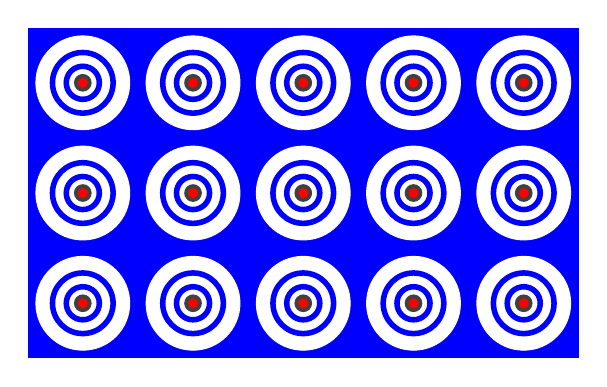
\begin{tikzpicture}[scale=0.7]
		
		\fill[blue] (1,1) rectangle (11,7);
		\draw[fill, white] (2,6) circle [radius=0.85];
		\draw[fill, white] (2,4) circle [radius=0.85];
		\draw[fill, white] (2,2) circle [radius=0.85];
		
		\draw[fill, white] (4,6) circle [radius=0.85];
		\draw[fill, white] (4,4) circle [radius=0.85];
		\draw[fill, white] (4,2) circle [radius=0.85];
		
		\draw[fill, white] (6,6) circle [radius=0.85];
		\draw[fill, white] (6,4) circle [radius=0.85];
		\draw[fill, white] (6,2) circle [radius=0.85];
		
		\draw[fill, white] (8,6) circle [radius=0.85];
		\draw[fill, white] (8,4) circle [radius=0.85];
		\draw[fill, white] (8,2) circle [radius=0.85];
		
		\draw[fill, white] (10,6) circle [radius=0.85];
		\draw[fill, white] (10,4) circle [radius=0.85];
		\draw[fill, white] (10,2) circle [radius=0.85];
		
		
		\draw[fill, darkgray] (2,6) circle [radius=0.15];
		\draw[fill, red] (2,6) circle [radius=0.08];
		\draw[blue, line width=2] (2,6) circle [radius=0.3];
		\draw[blue, line width=2] (2,6) circle [radius=0.55];
		\draw[fill, darkgray] (2,4) circle [radius=0.15];
		\draw[fill, red] (2,4) circle [radius=0.08];
		\draw[blue, line width=2] (2,4) circle [radius=0.3];
		\draw[blue, line width=2] (2,4) circle [radius=0.55];
		\draw[fill, darkgray] (2,2) circle [radius=0.15];
		\draw[fill, red] (2,2) circle [radius=0.08];
		\draw[blue, line width=2] (2,2) circle [radius=0.3];
		\draw[blue, line width=2] (2,2) circle [radius=0.55];
		
		\draw[fill, darkgray] (4,6) circle [radius=0.15];
		\draw[fill, red] (4,6) circle [radius=0.08];
		\draw[blue, line width=2] (4,6) circle [radius=0.3];
		\draw[blue, line width=2] (4,6) circle [radius=0.55];
		\draw[fill, darkgray] (4,4) circle [radius=0.15];
		\draw[fill, red] (4,4) circle [radius=0.08];
		\draw[blue, line width=2] (4,4) circle [radius=0.3];
		\draw[blue, line width=2] (4,4) circle [radius=0.55];
		\draw[fill, darkgray] (4,2) circle [radius=0.15];
		\draw[fill, red] (4,2) circle [radius=0.08];
		\draw[blue, line width=2] (4,2) circle [radius=0.3];
		\draw[blue, line width=2] (4,2) circle [radius=0.55];
		
		\draw[fill, darkgray] (6,6) circle [radius=0.15];
		\draw[fill, red] (6,6) circle [radius=0.08];
		\draw[blue, line width=2] (6,6) circle [radius=0.3];
		\draw[blue, line width=2] (6,6) circle [radius=0.55];
		\draw[fill, darkgray] (6,4) circle [radius=0.15];
		\draw[fill, red] (6,4) circle [radius=0.08];
		\draw[blue, line width=2] (6,4) circle [radius=0.3];
		\draw[blue, line width=2] (6,4) circle [radius=0.55];
		\draw[fill, darkgray] (6,2) circle [radius=0.15];
		\draw[fill, red] (6,2) circle [radius=0.08];
		\draw[blue, line width=2] (6,2) circle [radius=0.3];
		\draw[blue, line width=2] (6,2) circle [radius=0.55];
		
		\draw[fill, darkgray] (8,6) circle [radius=0.15];
		\draw[fill, red] (8,6) circle [radius=0.08];
		\draw[blue, line width=2] (8,6) circle [radius=0.3];
		\draw[blue, line width=2] (8,6) circle [radius=0.55];
		\draw[fill, darkgray] (8,4) circle [radius=0.15];
		\draw[fill, red] (8,4) circle [radius=0.08];
		\draw[blue, line width=2] (8,4) circle [radius=0.3];
		\draw[blue, line width=2] (8,4) circle [radius=0.55];
		\draw[fill, darkgray] (8,2) circle [radius=0.15];
		\draw[fill, red] (8,2) circle [radius=0.08];
		\draw[blue, line width=2] (8,2) circle [radius=0.3];
		\draw[blue, line width=2] (8,2) circle [radius=0.55];
		
		\draw[fill, darkgray] (10,6) circle [radius=0.15];
		\draw[fill, red] (10,6) circle [radius=0.08];
		\draw[blue, line width=2] (10,6) circle [radius=0.3];
		\draw[blue, line width=2] (10,6) circle [radius=0.55];
		\draw[fill, darkgray] (10,4) circle [radius=0.15];
		\draw[fill, red] (10,4) circle [radius=0.08];
		\draw[blue, line width=2] (10,4) circle [radius=0.3];
		\draw[blue, line width=2] (10,4) circle [radius=0.55];
		\draw[fill, darkgray] (10,2) circle [radius=0.15];
		\draw[fill, red] (10,2) circle [radius=0.08];
		\draw[blue, line width=2] (10,2) circle [radius=0.3];
		\draw[blue, line width=2] (10,2) circle [radius=0.55];
		\end{tikzpicture}
		\caption{Metallgitter Bohrsche Radien und Fermi-See} \label{fig:bandstr_metallg_b}
	\end{minipage}\par\medskip
\end{figure}

Typischerweise haben nun die quasi freien Elektronen im Fermi-See unterschiedliche kinetische Energien inne. Macht man einen Schnitt duch die Zeichnung und trägt die erlaubte Gesamtenergie des Elektrons im Kristall auf erhält man die Darstellugn in \ref{fig:bandstr_baender} (a). Um nun zum Halbleiter zu kommen muss man nur noch eine Bandlücke einführen, denn im Gegensatz zum Metall müssen Elektronen erst Energie zugeführt werden um vom Valenzband ins Leitungsband gehoben zu werden. Dies ist in Abbildung \ref{fig:bandstr_baender} (b) dargestellt. Wichtig dabei ist, dass das Valenzband durchgängig sein muss. Das lässt sich logisch damit begründen, da sonst ja keine Löcherleitung stattfinden könnte. Die eingefügte Bandlücke ist dann gerade die mittlere Energie die nötig ist um ein Elektron aus seiner kovalenten Bindung zu befreien.

\begin{figure}[H]
	\begin{minipage}{.5\linewidth}
		\centering
		\subfloat[]{\label{main:a}\includegraphics[scale=.3]{./img/bandstr_baender_metall.png}}
	\end{minipage}%
	\begin{minipage}{.5\linewidth}
		\centering
		\subfloat[]{\label{main:c}\includegraphics[scale=.3]{./img/bandstr_baender_hl.png}}
	\end{minipage}\par\medskip
	\caption{Besetzbare Zustände in 2D im Metall und Halbleiter \protect\cite{HL1}}
\label{fig:bandstr_baender}
\end{figure}

Zur Überprüfung dieses phänomenologisch hergeleiteten Modells liegt es nahe, den Kristall mit EM-Strahlung (hier weißes Licht) zu beschiessen. Mögliche Reaktionen des Kristalls sind Absorption, Transmission und Reflexion. 
\begin{itemize}
	\item In einem Metall stehen naturgemäß sehr viele freie Ladungsträger zur Verfügung, die direkt auf die einstrahlende EM-Welle reagieren. Hierbei werden die Elektronen durch die Welle in Schwingung versetzt, werden dadurch ihrerseits zu einem Hertzschen Dipol und emittieren eigens eine Welle. Damit sind beim Metall die Mechanismen Absorption und Reflexion gegeben. Eine Transmission findet durch die große Anzahl freier Ladungsträger praktisch nicht statt.
	\item Beim Halbleiter zeigt sich ein anders geartetes Verhalten. Da kaum intrinsische Ladungsträger zur Verfügung stehen die nicht erst ins Leitungsband angehoben werden müssen werden nur hoch energetische Wellen in Form einer Interbandanregung absorbiert. Der Rest transmittiert nahezu ungehindert durch den Kristall. Durch die Natur der Bandlücke ergibt sich eine sehr scharfe Absorptionskante bei einer bestimmten Frequenz.
\end{itemize}

Da nun die Struktur des Kristalls bekannt und nachgewiesen ist, stellt sich weiter die Frage über die Beweglichkeit der Elektronen/Löcher. Bei der Suche eines experimentellen Nachweises wurde der Hall-Effekt entdeckt. Hierbei wird an eine leitfähige Probe eine Spannung angelegt und ein Stromfluss durch die Probe angeregt. Senkrecht zu der Stromrichtung wird dann ein elektrisches Feld angelegt. Über das Feld werden die Ladungsträger abgelenkt so dass es zu einer einseitigen Ladungsträgerhäufung in der Probe kommt. Diese Ansammlung kann in Form einer Spannung gemessen werden. Daraus lässt sich leicht die Konzentration und Beweglichkeit bestimmen. Über das Vorzeichen der Hall-Spannung lässt sich weiter rausfinden ob es sich um Löcher oder Elektronen handelt.

\begin{figure}[H]
	\begin{center}
		\begin{tikzpicture}[scale=0.7]
	\draw[blue, thick] (2,2) rectangle (10,6);

		\draw[-, blue, thick] (2,6) to (3,7);
		\draw[-, blue, thick] (10,6) to (11,7);
		\draw[-, blue, thick] (10,2) to (11,3);
		
		\draw[-,blue,thick] (3,7) to (11,7);
		\draw[-,blue,thick] (11,3) to (11,7);
		
		\draw [dashed, blue, thick] (2,2) -- (3,3);
		\draw [dashed, blue, thick] (3,3) -- (3,7);
		\draw [dashed, blue, thick] (3,3) -- (11,3);
		
		\draw[fill, black](0,4.5) circle [radius=0.1];
		\draw[-, black, very thick] (0,4.5) to (2,4.5);
		\draw [dashed, black,very thick] (2,4.5) -- (2.5,4.5);
		\draw [dashed, black] (2.5,4.5) -- (10.5,4.5);
		\draw[fill, black](13,4.5) circle [radius=0.1];
		\draw[-Stealth, black, very thick] (10.5,4.5) to (12.95,4.5);
		
		\draw [dashed, black, very thick] (7.7,2) -- (7.7,7);
		\draw[-, black, very thick] (7.7,7) to (7.7,8);
		\draw[-, black, very thick] (7.7,8) to (6.49, 6.8);
		\draw[-, black, very thick] (6.5, 6.5) to (6.5, 6.8);
		\draw[-,black,very thick] (7.7, 2) to (6.7, 1);
		\draw[-,black,very thick] (6.7, 1) to (6.7,2);
		\draw[dashed,black,very thick] (6.7, 2) to (6.7,2.5);
		
		\draw[fill, white] (7.25, 1.5) circle [radius=0.35];
		\draw[black, very thick] (7.25, 1.5) circle [radius=0.35];
		\node at (7.25, 1.5) {V};
		\node at (7.75, 1.75) {+};
		\node at (7.05, 1.05) {-};
		
		\node at (0,5) {+};
		\node at (13,5) {-};
		\node at (1,5) {I};
		\draw[->, black] (0.8,4.7) to (1.2, 4.7);
		
		
		\draw[-,red,thick] (0.5, 3.5) to (2.5, 5.5);
		\draw[-,red,thick] (2.5, 3.5) to (4.5, 5.5);
		\draw[-,red,thick] (4.5, 3.5) to (6.5, 5.5);
		\draw[-,red,thick] (6.5, 3.5) to (8.5, 5.5);
		
		\draw[-,red,thick] (1.5, 1.5) to (3.5, 3.5);
		\draw[-,red,thick] (3.5, 1.5) to (5.5, 3.5);
		\draw[-,red,thick] (5.5, 1.5) to (7.5, 3.5);
		\draw[-,red,thick] (7.5, 1.5) to (9.5, 3.5);
		
		\draw[dashed, red,thick] (2.5, 5.5) to (4, 7);
		\draw[dashed, red,thick] (4.5, 5.5) to (6, 7);
		\draw[dashed, red,thick] (6.5, 5.5) to (8, 7);
		\draw[dashed, red,thick] (8.5, 5.5) to (10, 7);
		
		\draw[ -Stealth,red,thick] (4, 7) -- (4.5, 7.5);
		\draw[ -Stealth,red,thick] (6, 7) -- (6.5, 7.5);
		\draw[ -Stealth,red,thick] (8, 7) -- (8.5, 7.5);
		\draw[ -Stealth,red,thick] (10, 7) -- (10.5, 7.5);
		
		\draw[dashed, -Stealth,red,thick] (3.5, 3.5) -- (5.5, 5.5);
		\draw[dashed, -Stealth,red,thick] (5.5, 3.5) -- (7.5, 5.5);
		\draw[dashed, -Stealth,red,thick] (7.5, 3.5) -- (9.5, 5.5);
		\draw[dashed, -Stealth,red,thick] (9.5, 3.5) -- (11.5, 5.5);
		\end{tikzpicture}
	\end{center}
\end{figure}